\documentclass[11pt,a4paper]{scrartcl}

%\textwidth=15cm \hoffset=-1.2cm %
%\textheight=25cm \voffset=-2cm %
\pagestyle{headings}
%\parskip1ex

\date{}

\usepackage[T1]{fontenc} 
\usepackage[utf8]{inputenc} 
\usepackage[english]{babel} 
\usepackage{verbatim}
\usepackage{graphicx}
%\usepackage{amssymb}
\usepackage{acronym}
\usepackage{standalone}
\usepackage{url}
\usepackage{cite}
\usepackage{listings}
\usepackage{amsmath}
\usepackage{subcaption}
\usepackage{setspace}
%\usepackage[backend=bibtex]{biblatex}
%\setlength{\parskip}{\baselineskip}
\setlength{\parindent}{0pt}%
\onehalfspacing
\pagenumbering{arabic}

\def\keywords#1{\begin{center}{\bf Keywords}\\{#1}\end{center}} %

\def\titulo#1{\title{#1}} %
\def\autores#1{\author{#1}} %

%%%%%%%%%%%%%%%%%%%%%%%%%%%%%%%%%%%%%%%
\title{Evaluating Gossip-based aggregation\\{\LARGE An experimental study using network emulation}}
% Authors
\author{Niklas Semmler <semmler@kth.se>\\
Jiannan Guo <jiannang@kth.se>\\[0,25cm]
Supervisor: Prof. Maguire <maguire@kth.se>\\
KTH Royal Institute of Technology}%

\begin{document}
% Type down your paper title
%
\maketitle
\newcommand{\HRule}{\rule{\linewidth}{0.5mm}}
% This "." is necessary to let the line start on the left
%{.} \\
\noindent\HRule \\
\begin{abstract}
\noindent This study briefly introduces the gossip algorithm and aggregation mechanism. It addresses the influence of network topologies on the performance of a gossip-based aggregation algorithm. Several analytical studies are discussed. The hypothesis, the number of links is proportional to the convergence time, is evaluated. A basic gossip-based aggregation algorthm is implemented and its performance is determined in a network emulator. Four different network topologies serve as conditions. Data is collected from the experiment and the statistical method is utilized to test the hypothesis. The results support the hypothesis and a number of possible future extension become visible.
%TODO: add conclusion
\end{abstract}
\HRule \\
\keywords{Gossip-based aggregation, network emulation}% TODO: refine keywords

%\newpage
%\tableofcontents
%\newpage

%%%%%% Begin of Chapters %%%%%%%%

\section{Introduction}
\label{sec:theory}
% Introduction Sentence
With the increasing interconnection of all sorts of devices their management too becomes increasingly difficult. Large scale computer networks require solutions more scalable and reliable than what conventional centralized management can provide.

% Conventional algorithms and their disadvantages
Traditionally, variables of the network, such as throughput, workload and bandwidth, are gathered through the whole network by a central management system. Information is collected from all nodes of the network via periodic polling (e.g. SNMP) and stored in a database. Among several apparent drawbacks such as single point failure and performance bottleneck the most important is the inability to scale. A centralized management system cannot scale well with an increasing number of nodes, as any new node has to send its updates through the whole network. The load on the closer links increases with every additional node. In the long run this puts mission-critical business processes at risk \cite{Stadler529980}.

% Distributed algorithms as a super class
Distributed algorithms tackle these problems by propagating messages through the whole network in a more decentralized manner. Apart from dealing with the problems mentioned above they make global information locally accessible. Other components of the network can use this information to optimize their own behavior\cite{jelasity_gossip-based_2005}.

% Zooming in, the gossip algorithms
One variant of these algorithms is the Gossip-based aggregation. Gossip-based algorithms, also known as epidemic-style techniques \cite{I.Gupta2006}, are used to deal with drawback of deterministic algorithms in exchange for certainties. This algorithm is capable of aggregating global information in a completely decentralized manner \cite{jelasity_gossip-based_2005}. They differ from other distributed algorithms such as Echo algorithm proposed by Segell \cite{SegallG89} through their lack of structure. They do not require any structure of the network, other than an awareness of immediate neighbors. That said, gossip-based algorithms could be combined with tree-based algorithms to reach an optimization for some topologies \cite{KyasanurCG06}.

% The aspect we study network topology and it's influence on performance
It has previously been proven that the underlying network topology has a strong impact on the performance of gossip-based algorithm \cite{5929538, jelasity_gossip-based_2003}. Yet little work exist investigating the behavior of gossip-based aggregation in real network topologies. This study focuses on the divergence of performance in different topologies of real computer networks. To this purpose a number of networks, sharing the same number of nodes, have been chosen from an online database \cite{knight_internet_2011}.

% Goal -- UNCLEAR?!
Starting from the the problems of centralized management this study looks at the other side of the spectrum of management systems. This study aims at evaluating gossip-based aggregation in light of its dependence on network topology.

% An index of the paper
The remainder of the article is structured as follows. Section \ref{sec:theory} gives an introduction to the algorithm and our methodology. Next, section \ref{sec:implementation} presents the chosen implementation. Both the emulation of the networks and the implementation of the gossip algorithm are explained. Subsequently in section \ref{sec:result} the results of the experiment is presented. Conclusions and future work as well as related work is highlighted in section \ref{sec:conclusion}.

\documentclass[11pt,a4paper]{article}
\usepackage[T1]{fontenc} 
\usepackage[utf8]{inputenc}
\usepackage[english]{babel} 
\usepackage{verbatim}
\usepackage{graphicx}
\usepackage{acronym}
\usepackage{url}
\usepackage{cite}
\usepackage{amsmath}
\usepackage{tikz}
\usepackage{graphicx}

\begin{document}

\section{Chapter 2}
\subsection{Related work}
Motivated by peer-to-peer and {\it ad hoc} networks, a considerable number of studies have been done regarding gossip-based algorithms. Convergence and upper bound consensus time have been proved by J.Lavaei and R.Murray in \cite{5929538}. Analytical methods and simulations have been utilized to discuss the relations between performance of gossip protocols and topology of network, namely randomness, connectivity etc. As a subcategory of distributed algorithm, different models, such as synchronous and asynchronous models, with or without churn, are discussed in \cite{Lynch:1996:DA:525656}. The optimization of parameters of an asynchronous randomized gossip algorithm for fasted convergence is proved to be semi-definite problem \cite{Boyd2004}.\\
This study is mainly based on the work of M.Jelasity, A.Montresor and O.Babaoglu \cite{jelasity_gossip-based_2005}, focusing on existing static networks of different topologies \cite{knight_internet_2011}

\subsection{Gossip-based aggregation}
%TODO: describe the algorithm in details
\subsubsection{Gossip algorithm}
For better understanding of gossip algorithm, we assume a graph as in \ref{fig: epochs}.
\begin{figure}[!h]
   \begin{minipage}[t]{0.45\textwidth}
      \vspace{0pt}
      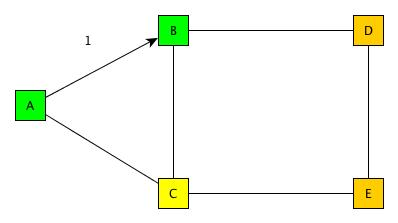
\includegraphics[width=\linewidth]{figures/network_gossip_1.jpg}
      Beginning of message dissemination (a)
   \end{minipage}
   \hfill
   \begin{minipage}[t]{0.45\textwidth}
      \vspace{0pt}
      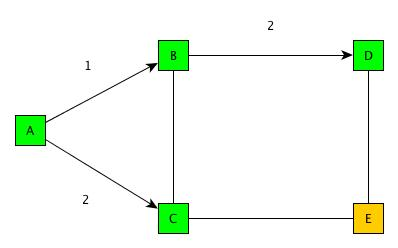
\includegraphics[width=\linewidth]{figures/network_gossip_2.jpg}
      Passing the message (b)
   \end{minipage}
   \vspace{5ex}
     \begin{center}
     \begin{minipage}[c]{0.45\textwidth}
      \vspace{0pt}
      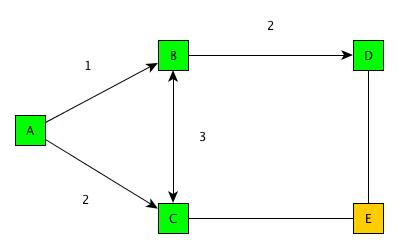
\includegraphics[width=\linewidth]{figures/network_gossip_3.jpg}
      Probable redundant message (c)
   	\end{minipage}
   \end{center}
   
   \caption{Gossip algorithm evolution epochs}
   \label{fig: epochs}
\end{figure}

Figure \ref{fig: epochs} illustrates a typical message dissemination process applying gossip algorithm. It starts with one node containing the information to be propagated, as in subgraph (a). It randomly chooses one neighbor and send the message. In second epoch, as showed in subgraph (b), this message is passed forward to next hop in the same manner, including the root node. By recursively applying same procedures, the message will be passed through the whole network eventually. Subgraph (c) shows the occurrence of probable redundant packet from node 3 to node 2, who's already aware of the message. Because of randomness of gossip algorithm, complete dissemination can only be achieved at a certain probability within given epochs, which can be denoted as $D(x)=\int_0^x P(\xi)\mathrm{d}\xi$\\

\subsubsection{Aggregation}
% TODO: illustrate aggregation

A simple implementation of synchronous gossip-based aggregation algorithm, inspired by \cite{jelasity_gossip-based_2005} can be illustrated by following pseudo code,
\begin{verbatim}
ActiveGossipThread
    for each consecutive *delta* time units at randomly picked time; do
        q <- GET_NEIGBOUR()
        send state_p to q
        state_q <- receive(q)
        state_p <- UPDATE(state_p, state_q)

PassiveGossipThread
    while true:
    state_q <- receive(*)
    send state_p to sender(state_q)
    state_p <- UPDATE(state_p, state_q)
\end{verbatim}

Although convergence is proved and expected convergence time can be estimated by probability density function for a certain topology \cite{5929538}, a drawback of probabilistic algorithm comparing to deterministic algorithm is reliability \cite{Lynch:1996:DA:525656}. The value can only be considered as true result at a certain probability. To put this protocol into practice, some extra procedures need to be added. In this study, we leave out the test of correctness inside implementation but try to obtain a empirical criteria according to the result of experiments.\\

\subsection{Impact of topology toward the performance of aggregation}
A plenty of methods exist to describe overlay topologies of a network, and different representations are used to describe properties of a topology. On the other hand, the performance of gossip-based aggregation is also abstracted differently for specific purpose.\\
In this study, we firstly focus on investigating the impact of various number of links with the number of nodes unchanged over the performance of gossip-based aggregation algorithm. Then we try to extract proper parameters representing a unweighted undirected connected graph through applying the definition of entropy presented by \cite{entropy1} and \cite{entropy2} and then we apply inductive research method \cite{portal} to address the relation between entropy and convergence time.
%TODO: describe definition in detail

\subsection{Applying to real network}
In order to apply control variable experiment method, we based our experiment on 4 real network topologies with same number of nodes (37) and different number of links, as showed in Table \ref{table: network}. Entropies are also calculated by applying methods presented by \cite{entropy1} (referred in the table as Entropy1) \cite{entropy2} (referred in the table as Entropy2).

\begin{table}
\centering
\begin{tabular}{lrrcrr}
	\hline
	Name of Network & Year & Country & \# of Links & Entropy1 & Entropy2\\
    \hline
    Reuna & 2010 & Chile & 36 & 202.0476 & 0.5164084\\
    BREN & 2010 & Bulgaria & 38 & 210.2229 & 0.6214745\\
    Geant & 2010 & Europe & 58 & 277.3282 & 1.530375\\
    Iij & 2010 & Japen, USA & 66 & 307.2482 & 1.553654\\
    \hline
\end{tabular}
\caption{Topologies under investigation}
\label{table: network}
\end{table}

\subsection{Hypothesis}
{\it Hypothesis 1.} In a given network topology $\mathcal{G}=\{\mathcal{E}, \mathcal{V}\}$, the number of links (edges) $N_E$ and convergence time $t$ are positively correlated, with number of nodes (vertices) $N_V$ unchanged.\\
{\it Hypothesis 2.} In a given network topology $\mathcal{G}=\{\mathcal{E}, \mathcal{V}\}$, the entropy of this graph $S$ and convergence time $t$ are positively correlated.

\subsection{Research methodology and methods}
We are creating a positivistic investigation grounded in quantitative experiments. With induction in the form of statistical inference, we aim to predict the behavior of the system under question in the boundary of our experimental research.\\
We clearly distinguish ourselves from realism, as we use network graphs inspired by real networks, but leave it to other research to prove that the experiment is representative of those real networks.\\
Since we will investigate several existing networks with the same number of nodes (constant) but different number of links (variable), we choose experimental research as our research method.\\
We will apply inductive reasoning research approach to verify the hypothesis. Since our unique contribution is an investigation of real network rather than a theoretical proof, deductive reasoning research approach won?t fit our goal properly. We will run our experiment multiple times to collect data and based on the observation of these phenomena we can obtain our conclusion.\\


\end{document}
\documentclass[11pt,a4paper]{article}
\usepackage[T1]{fontenc} 
\usepackage[utf8]{inputenc}
\usepackage[english]{babel} 
\usepackage{verbatim}
\usepackage{graphicx}
\usepackage{acronym}
\usepackage{url}
\usepackage{cite}
\usepackage{amsmath}

\begin{document}

\section{Chapter 3: Implementation}
\subsection{Simulation/Emulation of gossip-based aggregation}
To evaluate the value of the gossip-based aggregation it is necessary to see it in the wild of a real network environment. Unfortunately the setup of a real network is to time and cost intensive. Hence the next best thing was chosen: A network emulation. In a network simulation the network is simplified so as to illuminate a certain set of behaviours (e.g. ns \cite{ns}). An emulation in contrast consists of all the elements of the real network only that the resources are not "real" but "virtual". While for example an emulated switch may process network traffic in the very same way as a switch in your office, it could be implemented as a linux process.

In this research the netkit emulation framework (itself a wrapper to user mode linux \cite{uml}) was chosen. Netkit \cite{netkit} creates virtual linux machines from a set of configuration files. These virtual machines are automatically connected through usermode processes called "uml\_switch". It is possible to logon to the machines via ssh and configure them just like any other linux machines. This allows great freedom to try and test software which otherwise would be hard to implement.

The initial set of configuration files were created with the tool Autonetkit \cite{autonetkit} using network graphs from the "Topology Zoo" \cite{knight_internet_2011}. The "Topology Zoo" is a collection of around two hundred fifty graphs of telecommunication networks. The graphs are open for use and give a good idea on the reality of communication networks. Simon Knight, one of the founders of the topology zoo has developed the tool Autonetkit. It takes a graph xml file (graphml) and constructs over a series of abstractions configuration files (from OSPF to DNS). For the purpose of this experiment Autonetkit was augmented so as to create for our gossip agent a file containing all neighbours of the individual nodes.

\subsection{Implementation of gossip-based aggregation daemon}
As the gossip agent in our emulated network we developed a daemon based on the pseudo code of the gossip-based aggregation algorithm (REF: section 2 or article). The programming language Python \cite{python} was chosen for this task as it's simplicity and clarity enable a rapid development. Packets between nodes were exchanged in short lived TCP conections. The daemons on the individual nodes are started from outside the emulation system and write a log and results to the host system. After a number of periods (epochs) the daemons exit.

Two threads are coexisting (see figure \ref{fig:flow_diag}). The active thread connects to randomly chosen neighbours at a predefined interval (epoch duration). The passive thread accepts connection all the time. Each thread update a state after a succesful connection. To make the state develop linearly both threads have to compete for a lock before establishing a connection. (Combining multithreading with networking led to some problems, especially when two nodes chose to actively create a connection with each other at the same time.)
\begin{figure}[h!]
    \begin{center}
        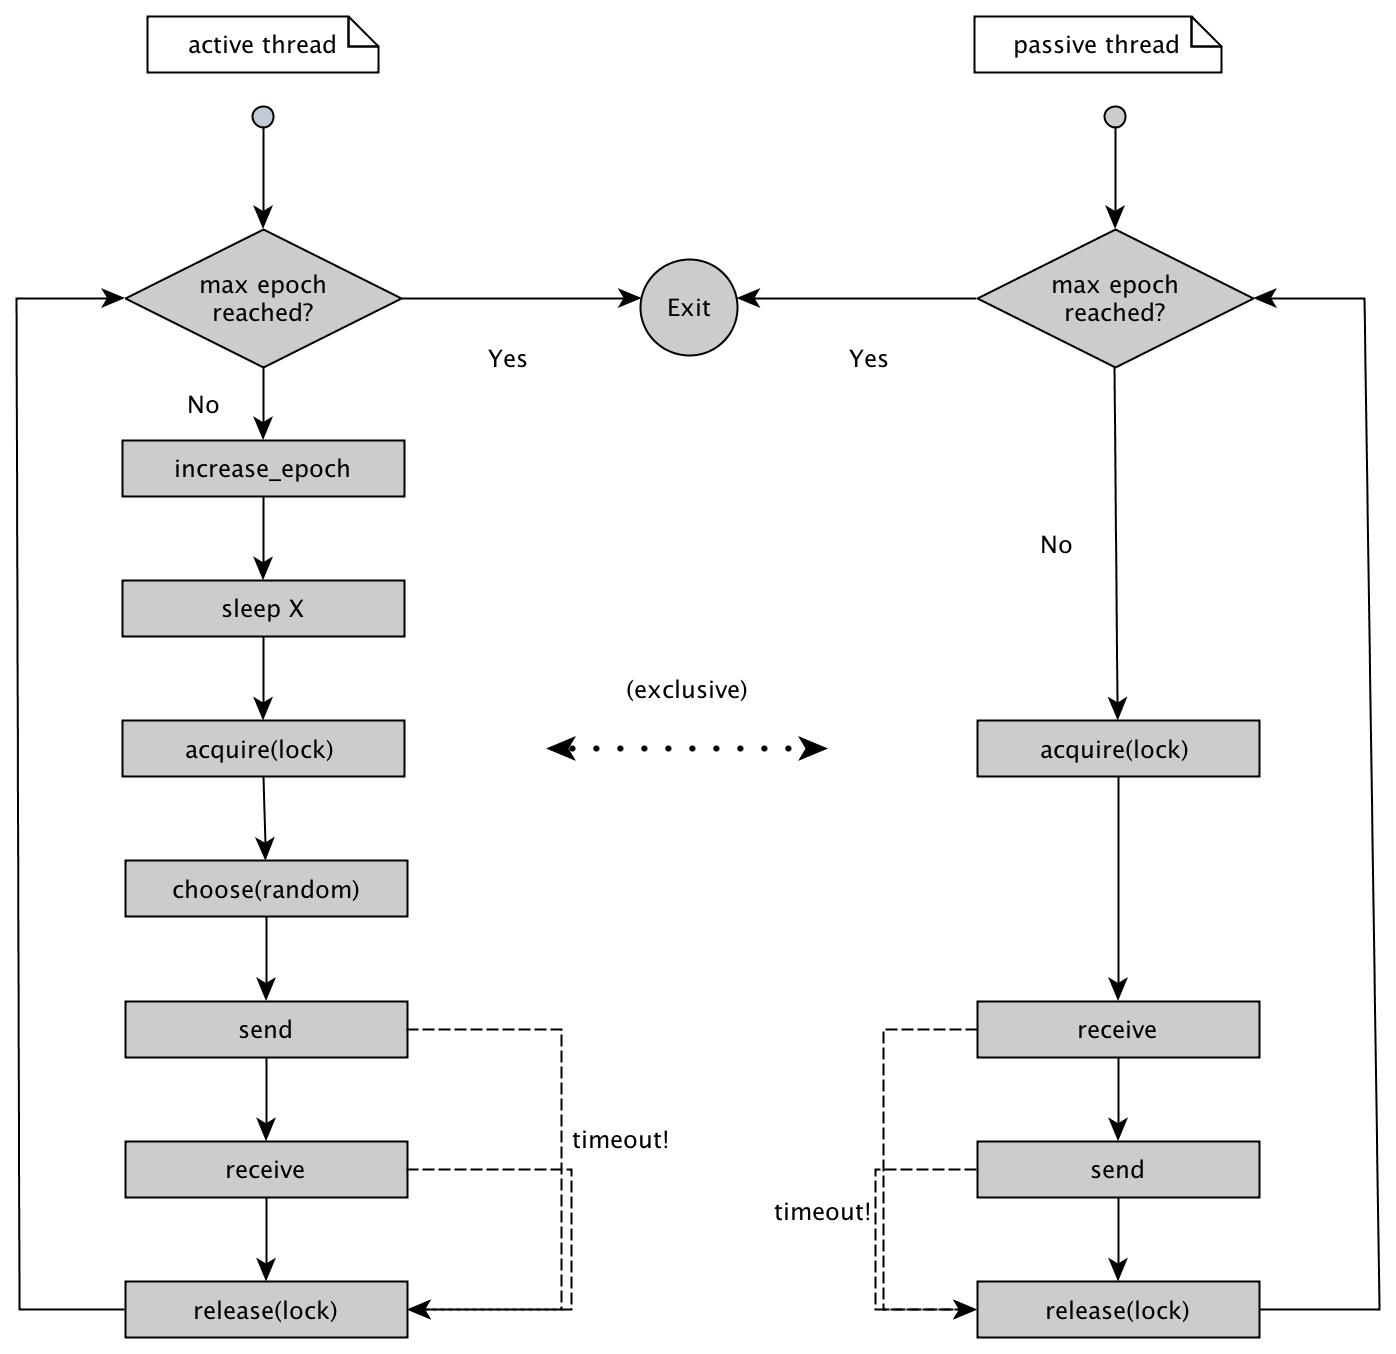
\includegraphics[scale=0.25]{flow_diag.jpg}
    \end{center}
    \caption{Flow diagram of the threads}
    \label{fig:flow_diag}
\end{figure}

Data created this way over one graph is analyzed in R. We compare our four different topologies (mentioned above) and visualize the results as charts.

\end{document}

\section{Results \& Discussion}
\label{sec:result}
\begin{figure}[h!]
	\centering
    \begin{minipage}[t]{0.47\textwidth}
    \vspace{0pt}
    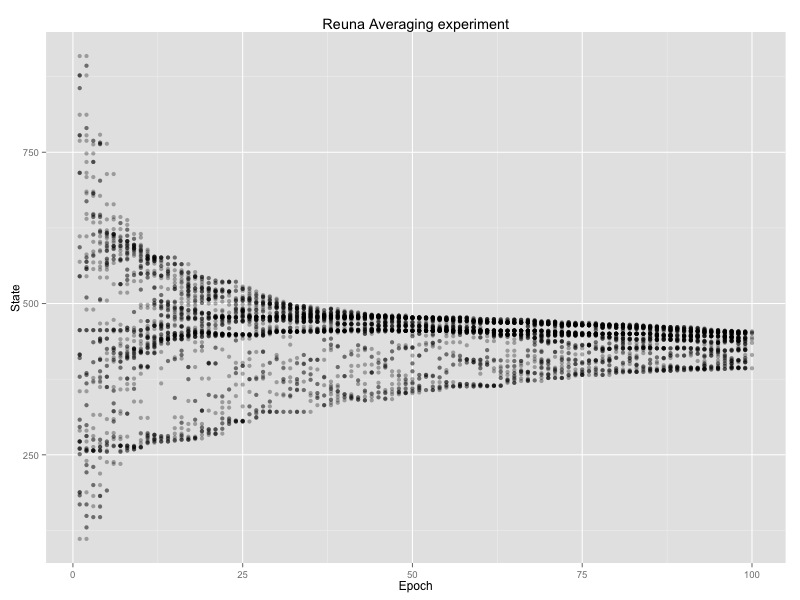
\includegraphics[width=\linewidth]{figures/Reuna.png}
    Reuna Averaging experiment
    \end{minipage}
    %\vspace{5ex}
    \begin{minipage}[t]{0.47\textwidth}
    \vspace{0pt}
    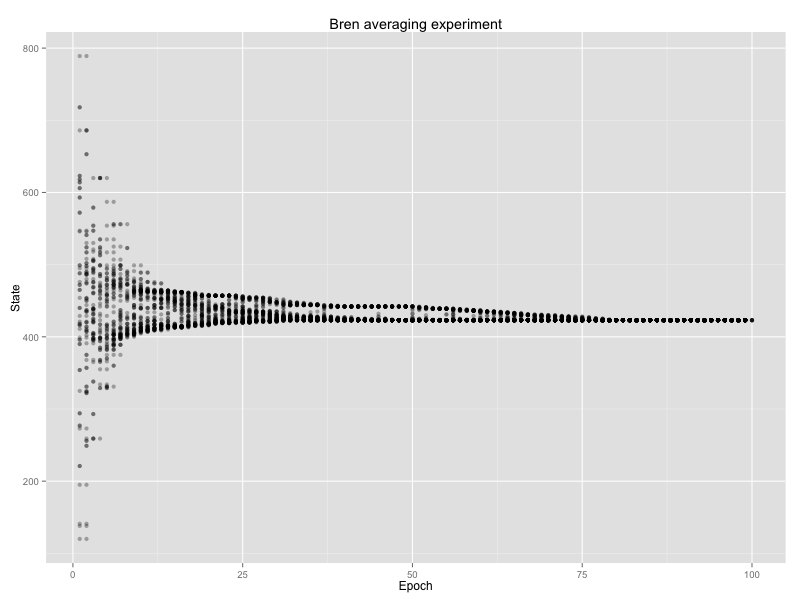
\includegraphics[width=\linewidth]{figures/Bren.png}
    Bren Averaging experiment
    \end{minipage}
    \vspace{5ex}
    \begin{minipage}[t]{0.47\textwidth}
    \vspace{0pt}
    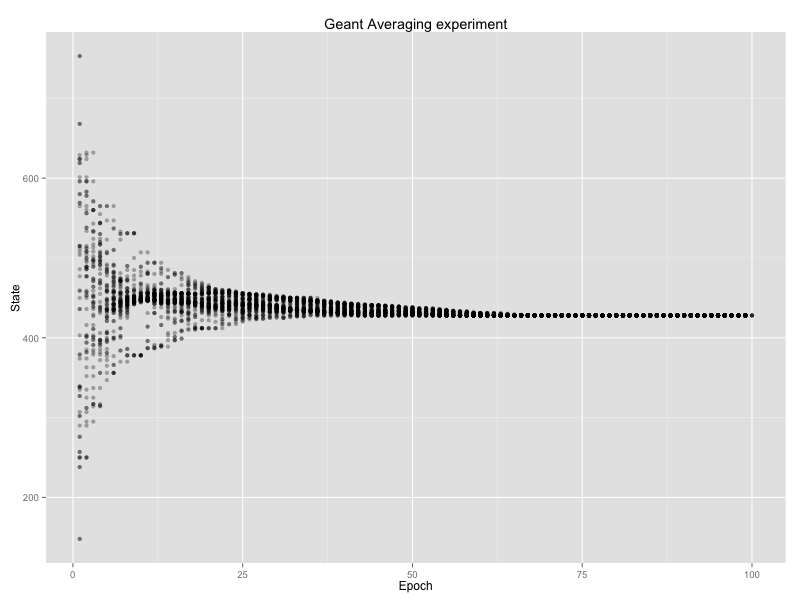
\includegraphics[width=\linewidth]{figures/Geant.png}
    Geant Averaging experiment
    \end{minipage}
    %\vspace{5ex}
    \begin{minipage}[t]{0.47\textwidth}
    \vspace{0pt}
    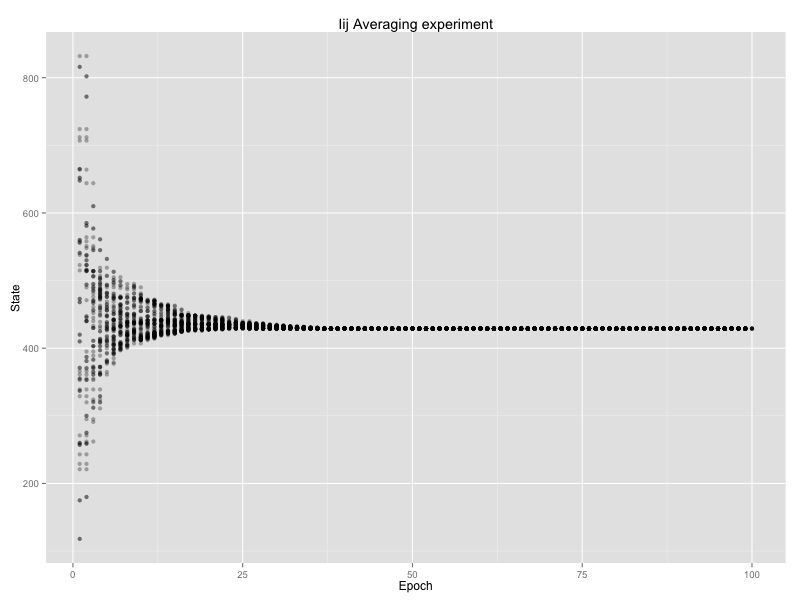
\includegraphics[width=\linewidth]{figures/Iij.png}
    Iij averaging experiment
    \end{minipage}
    \caption{State changes of all nodes per epoch}
    \label{fig:result}

\end{figure}
% aggregation of a random value from 0 to 1000
The results of our experiments are visualized in figure \ref{fig:result}. The X-axis are the epoch (time intervals) and the Y-axis is the state value. The gossip-based aggregation was run over 100 epochs. Every node started with a value chosen randomly between 0 and 1000. Due to the random nature of the algorithm and the difference in degree of connectivity among nodes a node can have between 1 and N state changes per epoch. (Where N is the amount of nodes in the network.) Overall nodes the number of state changes is 2*N per epoch. (Every node initiates one exchange per epoch which entails two state changes.) All of these changes are depicted.

The graphs are sorted according to number of links per nodes from left to right and top to bottom. Inside 100 epochs all four experiments are in the trend of converging and if we set convergence criteria as 5\% of mean value, Bren, Geant and Iij converge inside their run of experiments, accordingly at the 75th, 60th and the 40th epoch. Reuna does not converge during the 100 epochs of our experiment.

Thus, the order of convergence speed can be derived as Iij, Geant, Bren, Reuna, from the fastest to slowest, which supports our hypothesis.

\begin{figure}[h!]
    \begin{center}
    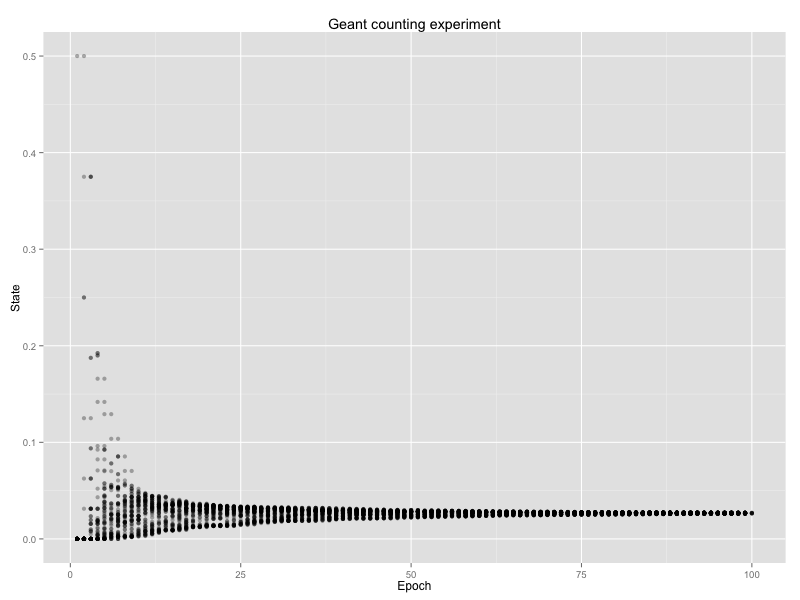
\includegraphics[scale=0.4]{figures/geant_counting_exp.png}
    \end{center}
    \caption{Geant counting}
    \label{fig:geant}
\end{figure}
\label{sec:results}

\documentclass[11pt,a4paper]{article}
\usepackage[T1]{fontenc} 
\usepackage[utf8]{inputenc}
\usepackage[english]{babel} 
\usepackage{verbatim}
\usepackage{graphicx}
\usepackage{acronym}
\usepackage{url}
\usepackage{cite}
\usepackage{amsmath}

\begin{document}
\newpage

\section{Future works}

\subsection{More comprehensive emulation}

\subsection{Relation between the performance and other properties of graph}

%%% put into future work %%%
In \cite{jelasity_gossip-based_2005}, convergence factor $E(2^{-\phi})$ is used to determine convergence time, smaller convergence factor results in faster convergence. The Watts-Strogatz is used to model the topology of overlay network, indicating randomness as an independent variable \cite{Watts1998}. Thus, a function is derived, with randomness parameter $\beta$ as input and convergence factor $E(2^{-\phi})$ as output.
%%%%%%%%%%%%%%%%%%%%%%%%%%%%

\end{document}

%%%%%% End of Chapters %%%%%%%%%%

\bibliographystyle{ieeetr}
\bibliography{report}

\appendix


\end{document}
